% --- Aufgabenblatt: Geometrische Berechnungen von Prismen ---

\section*{Aufgabenblatt: Geometrische Berechnungen von Prismen}

\subsection*{1. Grundlagen}
\textbf{a)} Erklären Sie, was ein Prisma ist. Welche Eigenschaften besitzt ein gerades Prisma?

\textbf{b)} Nennen Sie drei Beispiele für Prismen aus dem Alltag und beschreiben Sie deren Grundfläche.

\subsection*{2. Skizzen und Bezeichnungen}
\textbf{a)} Zeichnen Sie ein gerades dreieckiges Prisma mit den Kantenlängen $a=4\,\mathrm{cm}$, $b=3\,\mathrm{cm}$, $c=5\,\mathrm{cm}$ und der Höhe $h=6\,\mathrm{cm}$. Beschriften Sie die Kanten und die Höhe.

\begin{center}
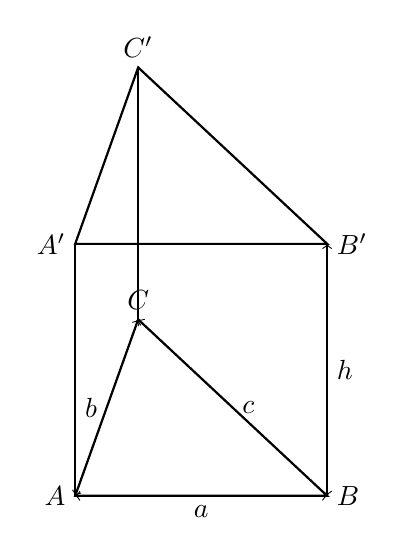
\begin{tikzpicture}[scale=0.8]
  % Grundfläche
  \coordinate (A) at (0,0);
  \coordinate (B) at (4,0);
  \coordinate (C) at (1,2.8);
  % Deckfläche
  \coordinate (A') at (0,4);
  \coordinate (B') at (4,4);
  \coordinate (C') at (1,6.8);
  % Grundfläche
  \draw[thick] (A) -- (B) -- (C) -- cycle;
  % Deckfläche
  \draw[thick] (A') -- (B') -- (C') -- cycle;
  % Seitenkanten
  \draw[thick] (A) -- (A');
  \draw[thick] (B) -- (B');
  \draw[thick] (C) -- (C');
  % Beschriftungen
  \node[left] at (A) {$A$};
  \node[right] at (B) {$B$};
  \node[above] at (C) {$C$};
  \node[left] at (A') {$A'$};
  \node[right] at (B') {$B'$};
  \node[above] at (C') {$C'$};
  % Kanten
  \draw[<->] (A) -- node[below] {$a$} (B);
  \draw[<->] (B) -- node[right] {$c$} (C);
  \draw[<->] (C) -- node[left] {$b$} (A);
  % Höhe
  \draw[<->,dashed] (B) -- node[right] {$h$} (B');
\end{tikzpicture}
\end{center}

\textbf{b)} Benennen Sie in Ihrer Skizze die Grundfläche, die Deckfläche und eine Seitenfläche.

\subsection*{3. Volumen- und Oberflächenberechnung}
\textbf{a)} Ein gerades rechteckiges Prisma hat die Grundfläche $A=5\,\mathrm{cm} \times 3\,\mathrm{cm}$ und die Höhe $h=8\,\mathrm{cm}$. Berechnen Sie das Volumen und die gesamte Oberfläche. Geben Sie alle Zwischenschritte an.

\textbf{b)} Ein dreieckiges Prisma hat als Grundfläche ein rechtwinkliges Dreieck mit den Katheten $a=6\,\mathrm{cm}$ und $b=8\,\mathrm{cm}$. Die Höhe des Prismas beträgt $h=10\,\mathrm{cm}$. Berechnen Sie das Volumen und die Oberfläche.

\textbf{c)} Ein regelmäßiges sechseckiges Prisma hat eine Seitenlänge von $a=2\,\mathrm{cm}$ und eine Höhe von $h=9\,\mathrm{cm}$. Berechnen Sie das Volumen. (Hinweis: Die Fläche eines regelmäßigen Sechsecks mit Seitenlänge $a$ ist $A=\frac{3\sqrt{3}}{2}a^2$)

\subsection*{4. Anwendungsaufgaben}
\textbf{a)} Ein Aquarium hat die Form eines rechteckigen Prismas mit den Maßen $60\,\mathrm{cm} \times 30\,\mathrm{cm} \times 40\,\mathrm{cm}$. Wie viel Liter Wasser passen maximal hinein? (1 Liter = 1000 $\mathrm{cm}^3$)

\textbf{b)} Ein Zelt hat die Form eines dreieckigen Prismas. Die Grundfläche ist ein gleichschenkliges Dreieck mit Basis $b=3\,\mathrm{m}$ und Höhe $h_\text{Dreieck}=2\,\mathrm{m}$. Die Länge des Zeltes beträgt $l=4\,\mathrm{m}$. Berechnen Sie das Volumen des Zeltes.

\textbf{c)} Ein Glasprisma hat die Form eines regelmäßigen dreieckigen Prismas mit Seitenlänge $a=2\,\mathrm{cm}$ und Höhe $h=10\,\mathrm{cm}$. Wie viel $\mathrm{cm}^3$ Glas werden benötigt?

\subsection*{5. Zusatzaufgaben mit Skizze}
\textbf{a)} Zeichnen Sie ein regelmäßiges sechseckiges Prisma mit Höhe $h=5\,\mathrm{cm}$ und Seitenlänge $a=2\,\mathrm{cm}$. Beschriften Sie die wichtigsten Maße und markieren Sie eine Seitenfläche farbig.

\begin{center}
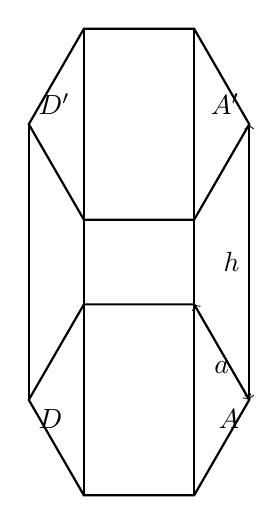
\begin{tikzpicture}[scale=0.7]
  \foreach \i in {0,...,5} {
    \coordinate (G\i) at ({2*cos(60*\i)},{2*sin(60*\i)});
    \coordinate (H\i) at ({2*cos(60*\i)},{2*sin(60*\i)+5});
  }
  % Grundfläche
  \draw[thick] (G0) \foreach \i in {1,...,5} {-- (G\i)} -- cycle;
  % Deckfläche
  \draw[thick] (H0) \foreach \i in {1,...,5} {-- (H\i)} -- cycle;
  % Seitenkanten
  \foreach \i in {0,...,5} {
    \draw[thick] (G\i) -- (H\i);
  }
  % Beschriftungen
  \node[below left] at (G0) {$A$};
  \node[below right] at (G3) {$D$};
  \node[above left] at (H0) {$A'$};
  \node[above right] at (H3) {$D'$};
  % Seitenlänge
  \draw[<->] (G0) -- node[below] {$a$} (G1);
  % Höhe
  \draw[<->,dashed] (G0) -- node[left] {$h$} (H0);
\end{tikzpicture}
\end{center}

% --- Ende des Aufgabenblatts ---